\documentclass{beamer}
\usepackage{pgfpages}
\usepackage[utf8]{inputenc}
\usepackage{times}
\usepackage{tikz}
\usetheme{Warsaw}
\setbeamercovered{transparent}
\useoutertheme{infolines}
\setbeamertemplate{footline} [frame number]
\title{Automatic identification of landmarks by shape recognition}
\author{LE Van Linh}
<<<<<<< HEAD

\date{Oct 29, 2015}
=======
%\institute{LaBRI laboratory}
\date{\today}
>>>>>>> 3a74f3884c9b984ff6b816654ee1c30026afb51d
\begin{document}
\frame{\titlepage}
\begin{frame}{Contents}
	\tableofcontents
\end{frame}
\section{Introduction}
\begin{frame}{Introduction}
	\begin{itemize}
		\item Shape analysis by landmarks is increasingly used in biological and medical applications.
		\item Indicate the landmarks:
			\begin{itemize}
				\item By hands
				\item Automatically
			\end{itemize}			  
	\end{itemize}
\end{frame}
\begin{frame}{Introduction}
	The propose method$^{\cite{palaniswamy}}$ includes four steps:
	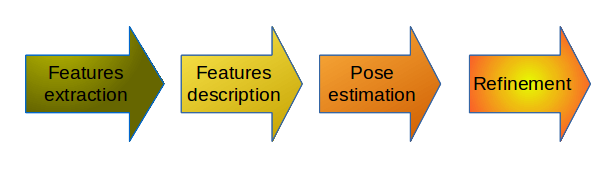
\includegraphics[height=3.5cm]{images/flow.png}
\end{frame}
\section{Method}
\subsection{Segmentation}
\begin{frame}{Segmentation}
	Purpose: 
	\begin{itemize}
		\item Extract the features (edge) from images
		\item Get the approximate lines
	\end{itemize}
	Method:
	\begin{itemize}
		\item Indicate the threshold value by analysis histogram of image		
		\item Canny
		\item Break edge algorithm
	\end{itemize}
	Result: The set of approximate lines
\end{frame}
\subsection{Pairwise geometric histogram(PGH)}
\begin{frame}{Pairwise geometric histogram}
	\begin{description}
		\item[Purpose:] detecting the present of scene image in model image
		\item[Method$^{\cite{pgh}}$:]
		\begin{itemize}
			\item Construct the local PGH
			\item Construct the shape PGH
			\item Matching shape's PGH by Bhattacharyya metric
		\end{itemize}
	\end{description}
\end{frame}
\begin{frame}{Pairwise geometric histogram}
	\framesubtitle{Local PGH and shape PGH}
	\begin{description}
		\item[Local PGH]: PGH for each feature (line)
		\item[Shape PGH]: contains many \textbf{Local PGH}
		\item[PGH]: a matrix two dimensions: angle axis and distance axis
		\item[PGH information]: angle between two lines and perpendicular distance from two endpoints of scene line to reference line.
	\end{description}
\end{frame}
\subsection{Probabilistic Hough Transform}
\begin{frame}{Probabilistic Hough Transform}
	\begin{description}
		\item[Purpose:]
			\begin{itemize}
				\item Determine the presence and location of model image in scene image
				\item Estimate the landmarks in the scene image
			\end{itemize}
		\item[Method:]
		\begin{itemize}
			\item Construct the reference table
			\item Find the pair scene lines have the best ``vote"
			\item Estimate the ``reference point" in scene image
			\item Estimate the landmarks
		\end{itemize}
		\item[Result:] Estimated model landmarks on scene image
	\end{description}
\end{frame}
\begin{frame}{Probabilistic Hough Transform}
	\begin{columns}[c]
		\column{0.5\textwidth}
		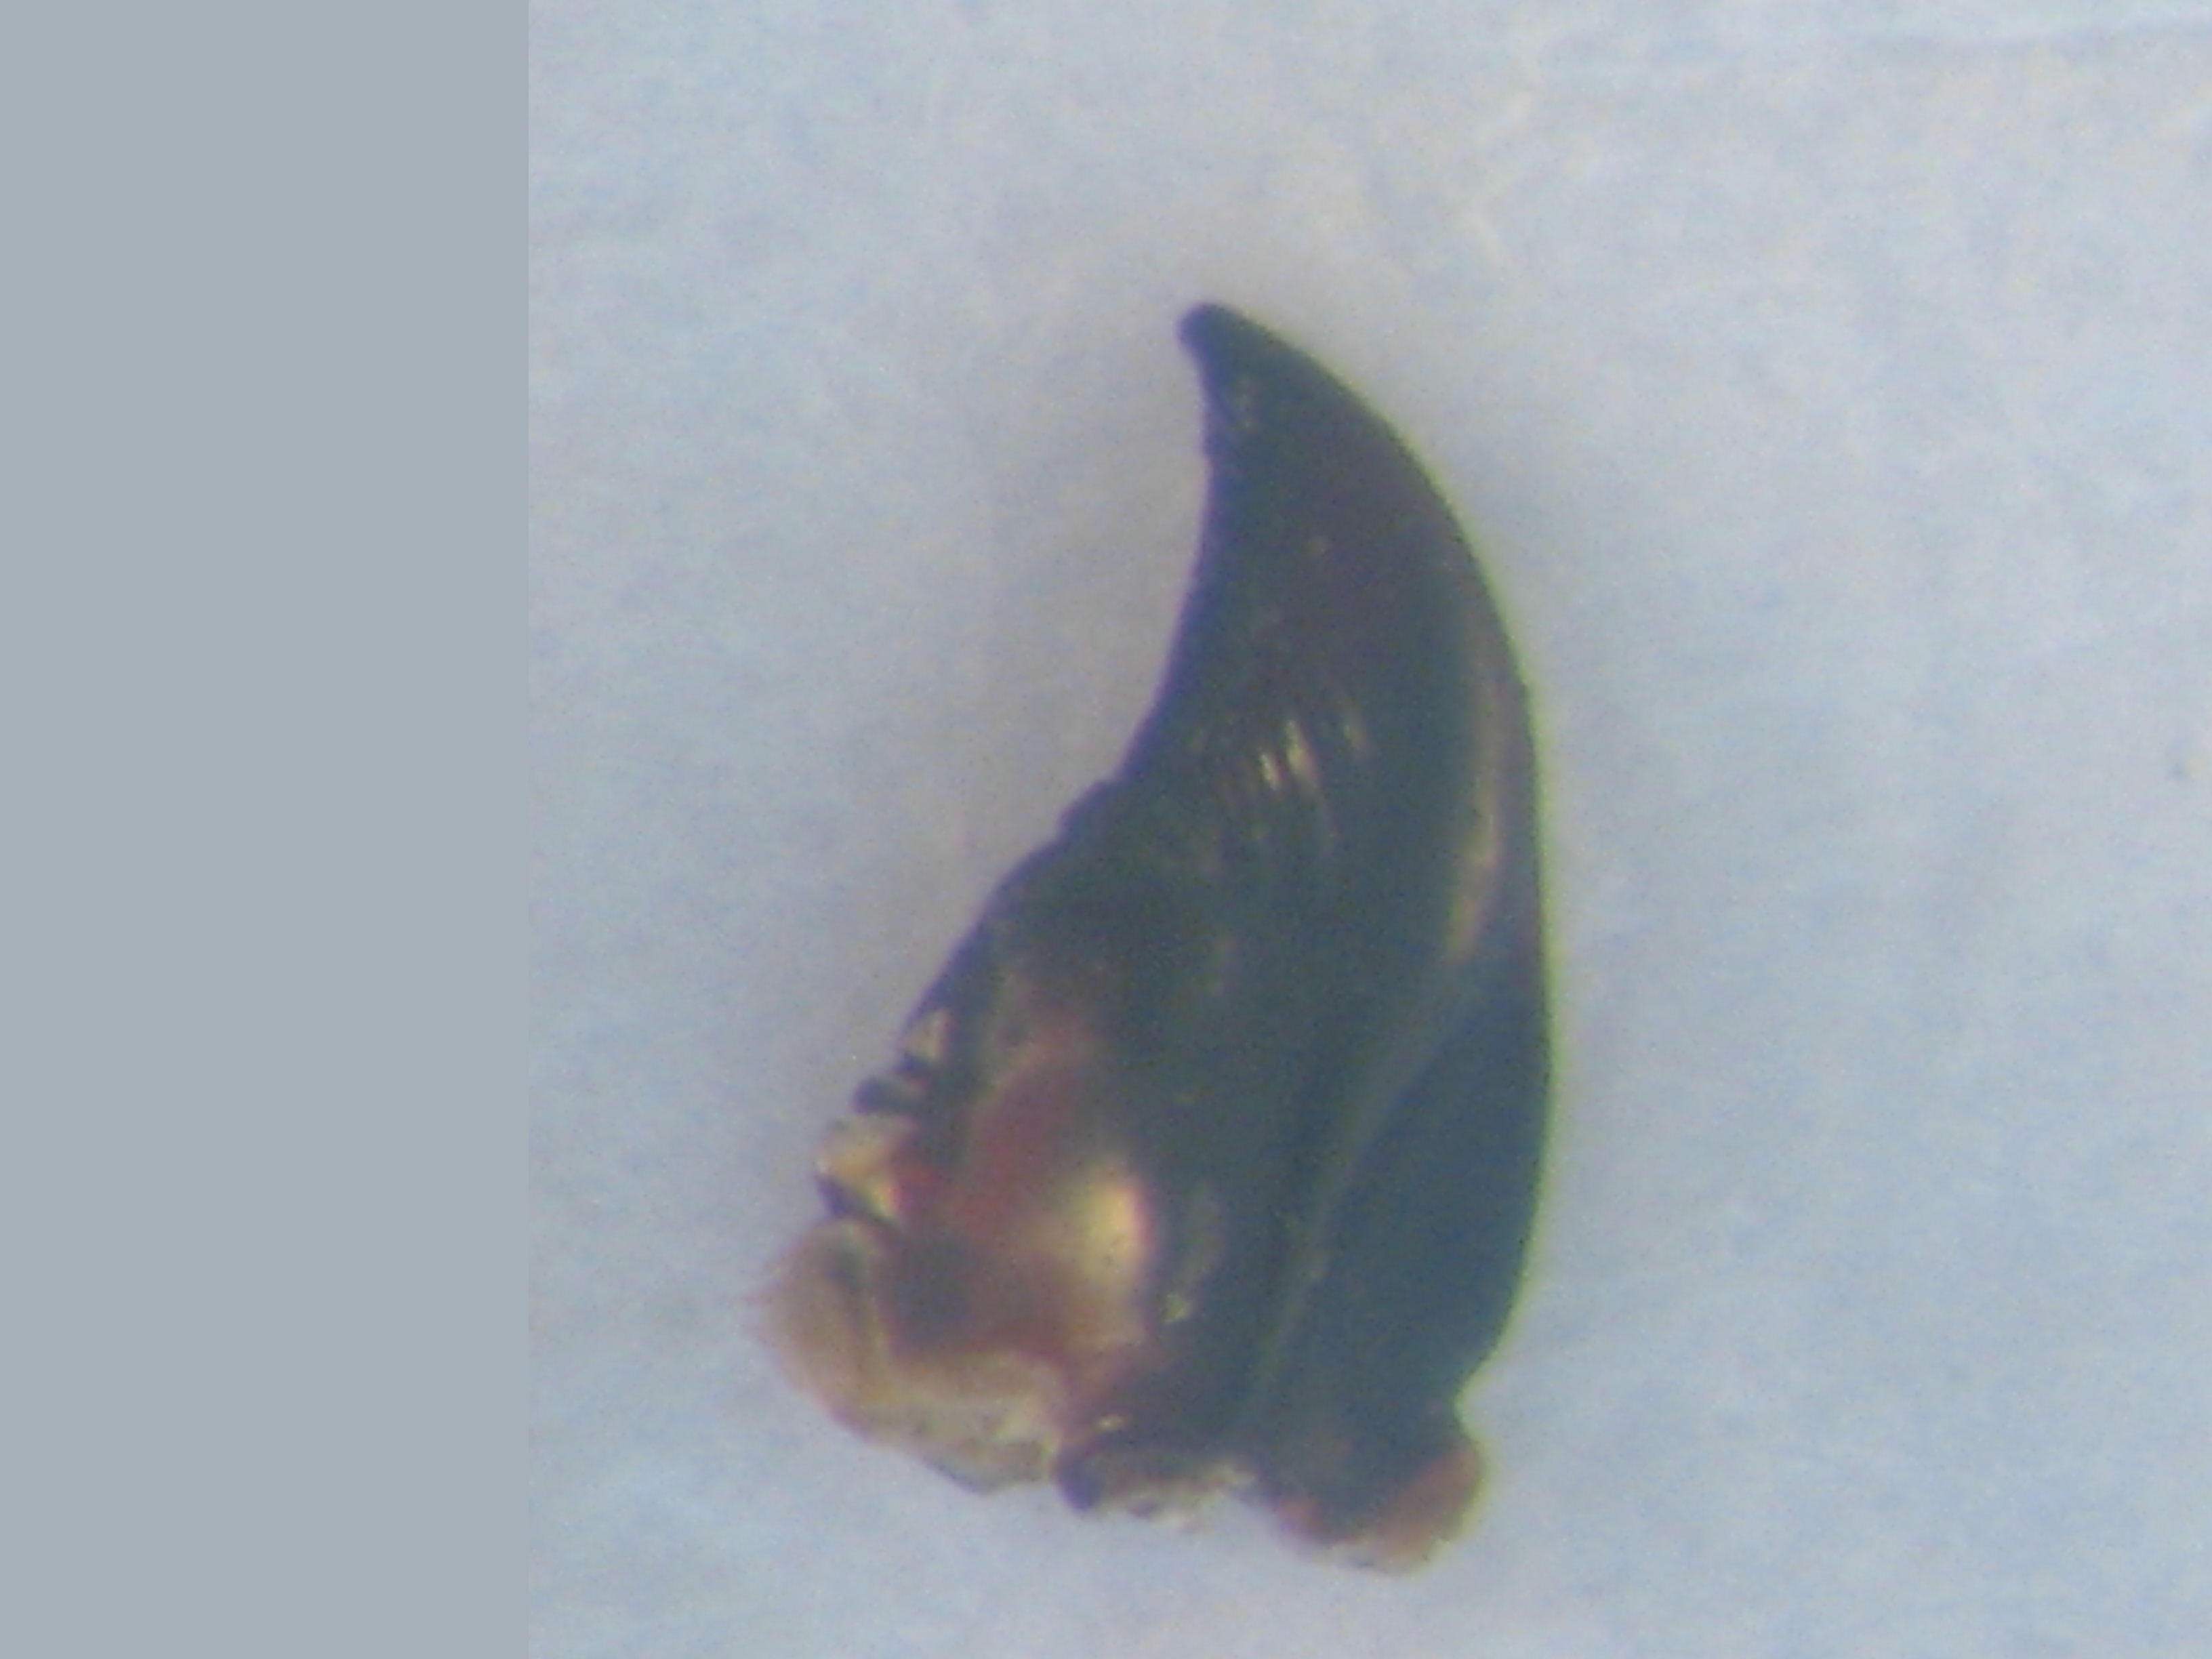
\includegraphics[height=4.5cm]{images/model28.JPG}
		\column{0.5\textwidth}
		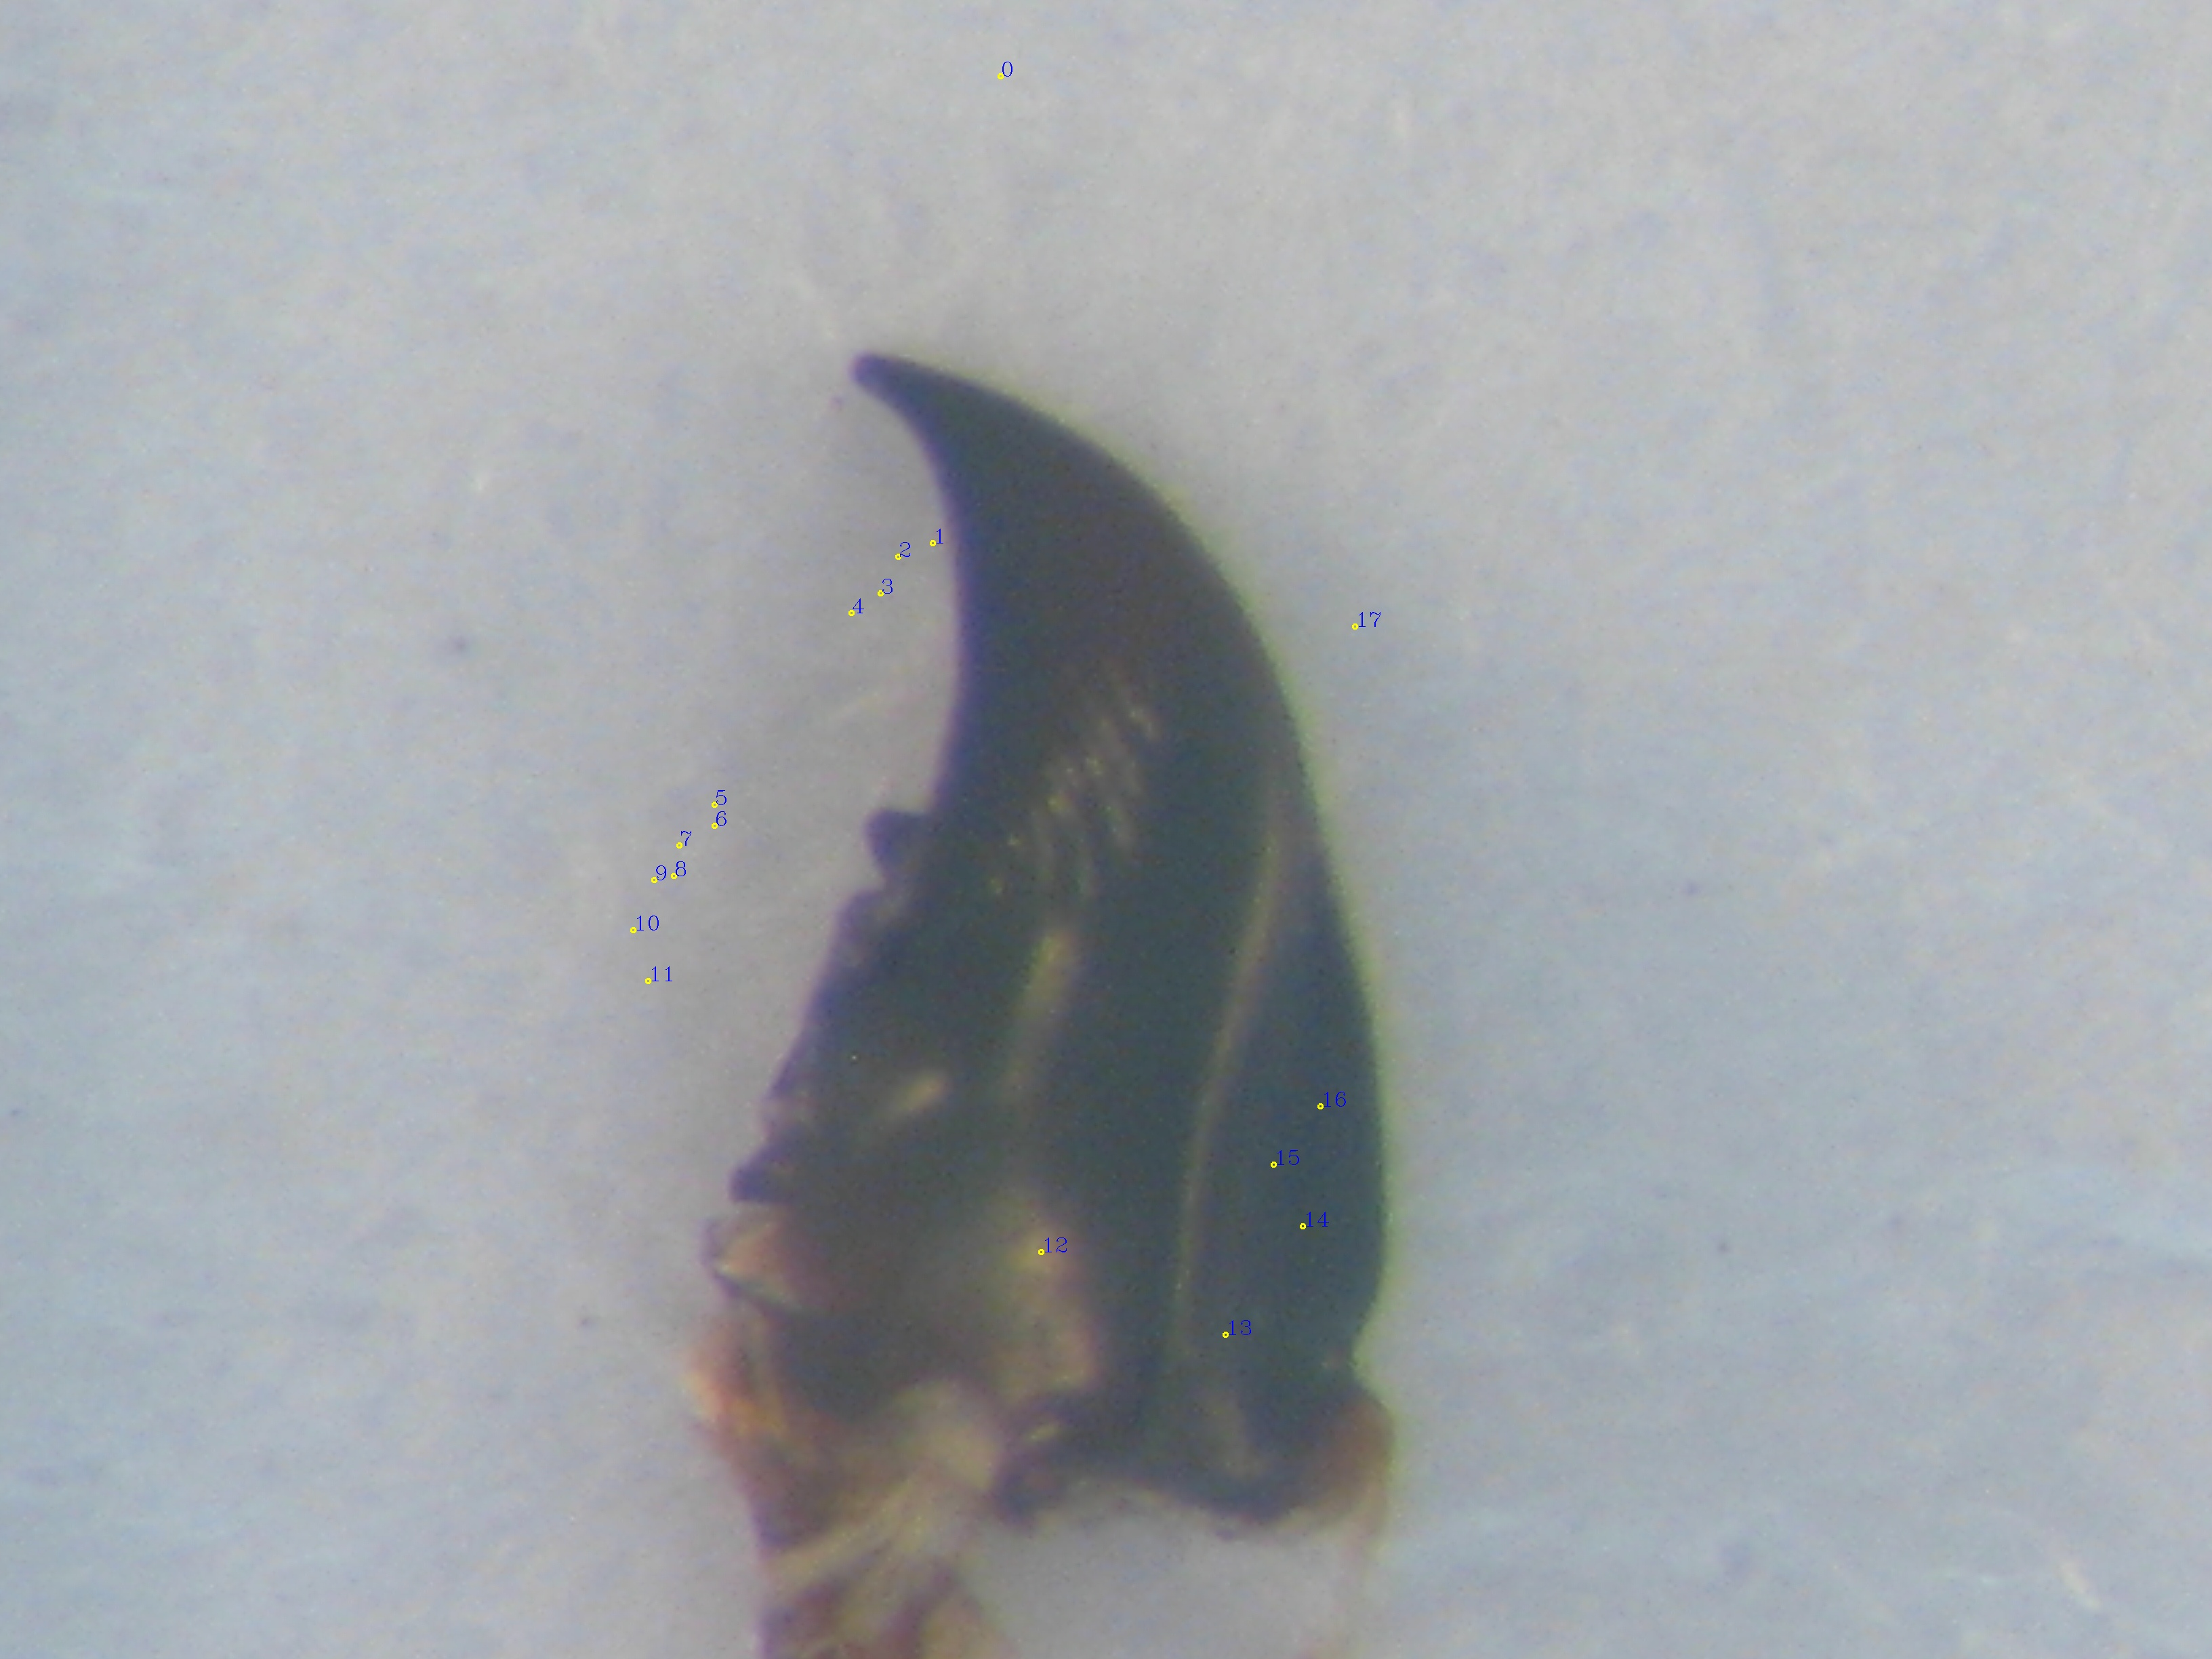
\includegraphics[height=4.5cm]{images/pht32.JPG}
	\end{columns}
\end{frame}
\subsection{Template matching}
\begin{frame}{Template matching}
	\begin{description}
		\item [Purpose:] Refine the estimated landmarks on the scene image 
		\item [Method:] 
			\begin{itemize}
				\item On model image: For each landmark, create a bounding box with size ``\textit{t1}" and \textit{landmark} is center point of box
				\item Rotate scene image to match with model
				\item On scene image: For each estimated landmark, create a bounding box with size ``\textit{t2}" and \textit{landmark} is center point of box
				\item Sliding \textit{t1} on \textit{t2} and find the the best match (cross-correlation)
			\end{itemize}
	\end{description}
\end{frame}
\begin{frame}{Template matching}
	\begin{columns}[c]
		\column{0.5\textwidth}
		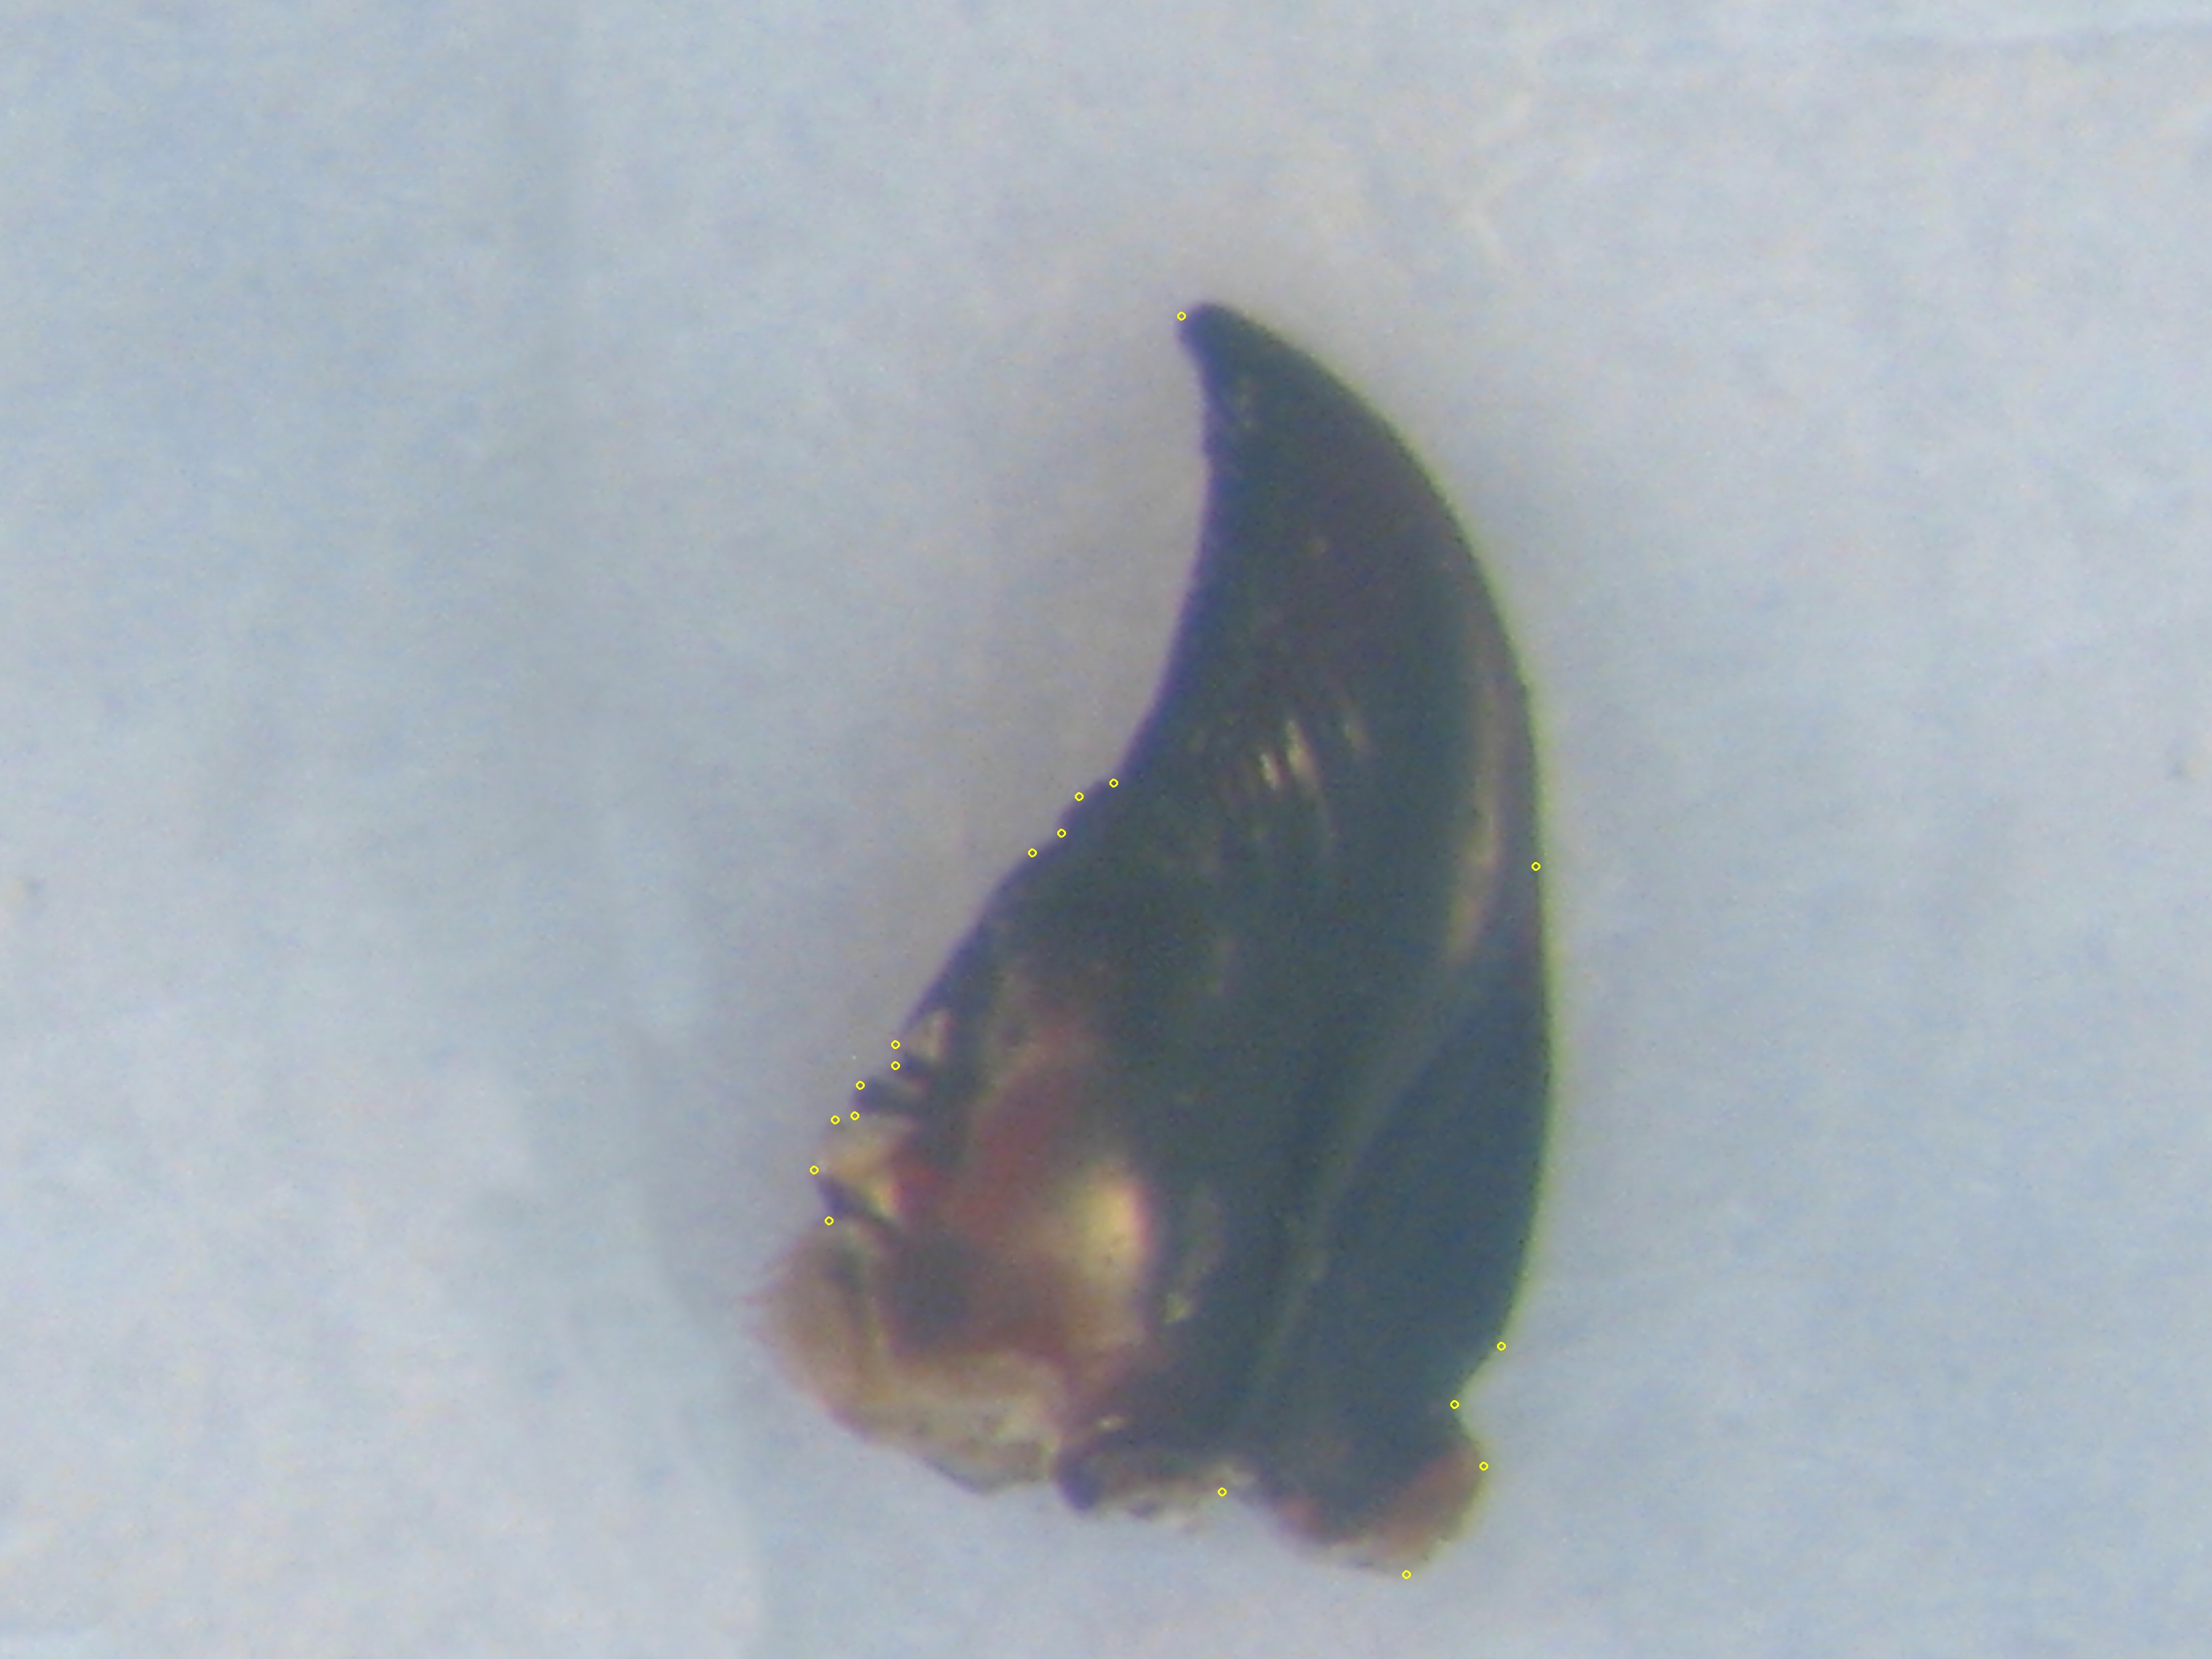
\includegraphics[height=4.5cm]{images/est28.JPG}
		\column{0.5\textwidth}
		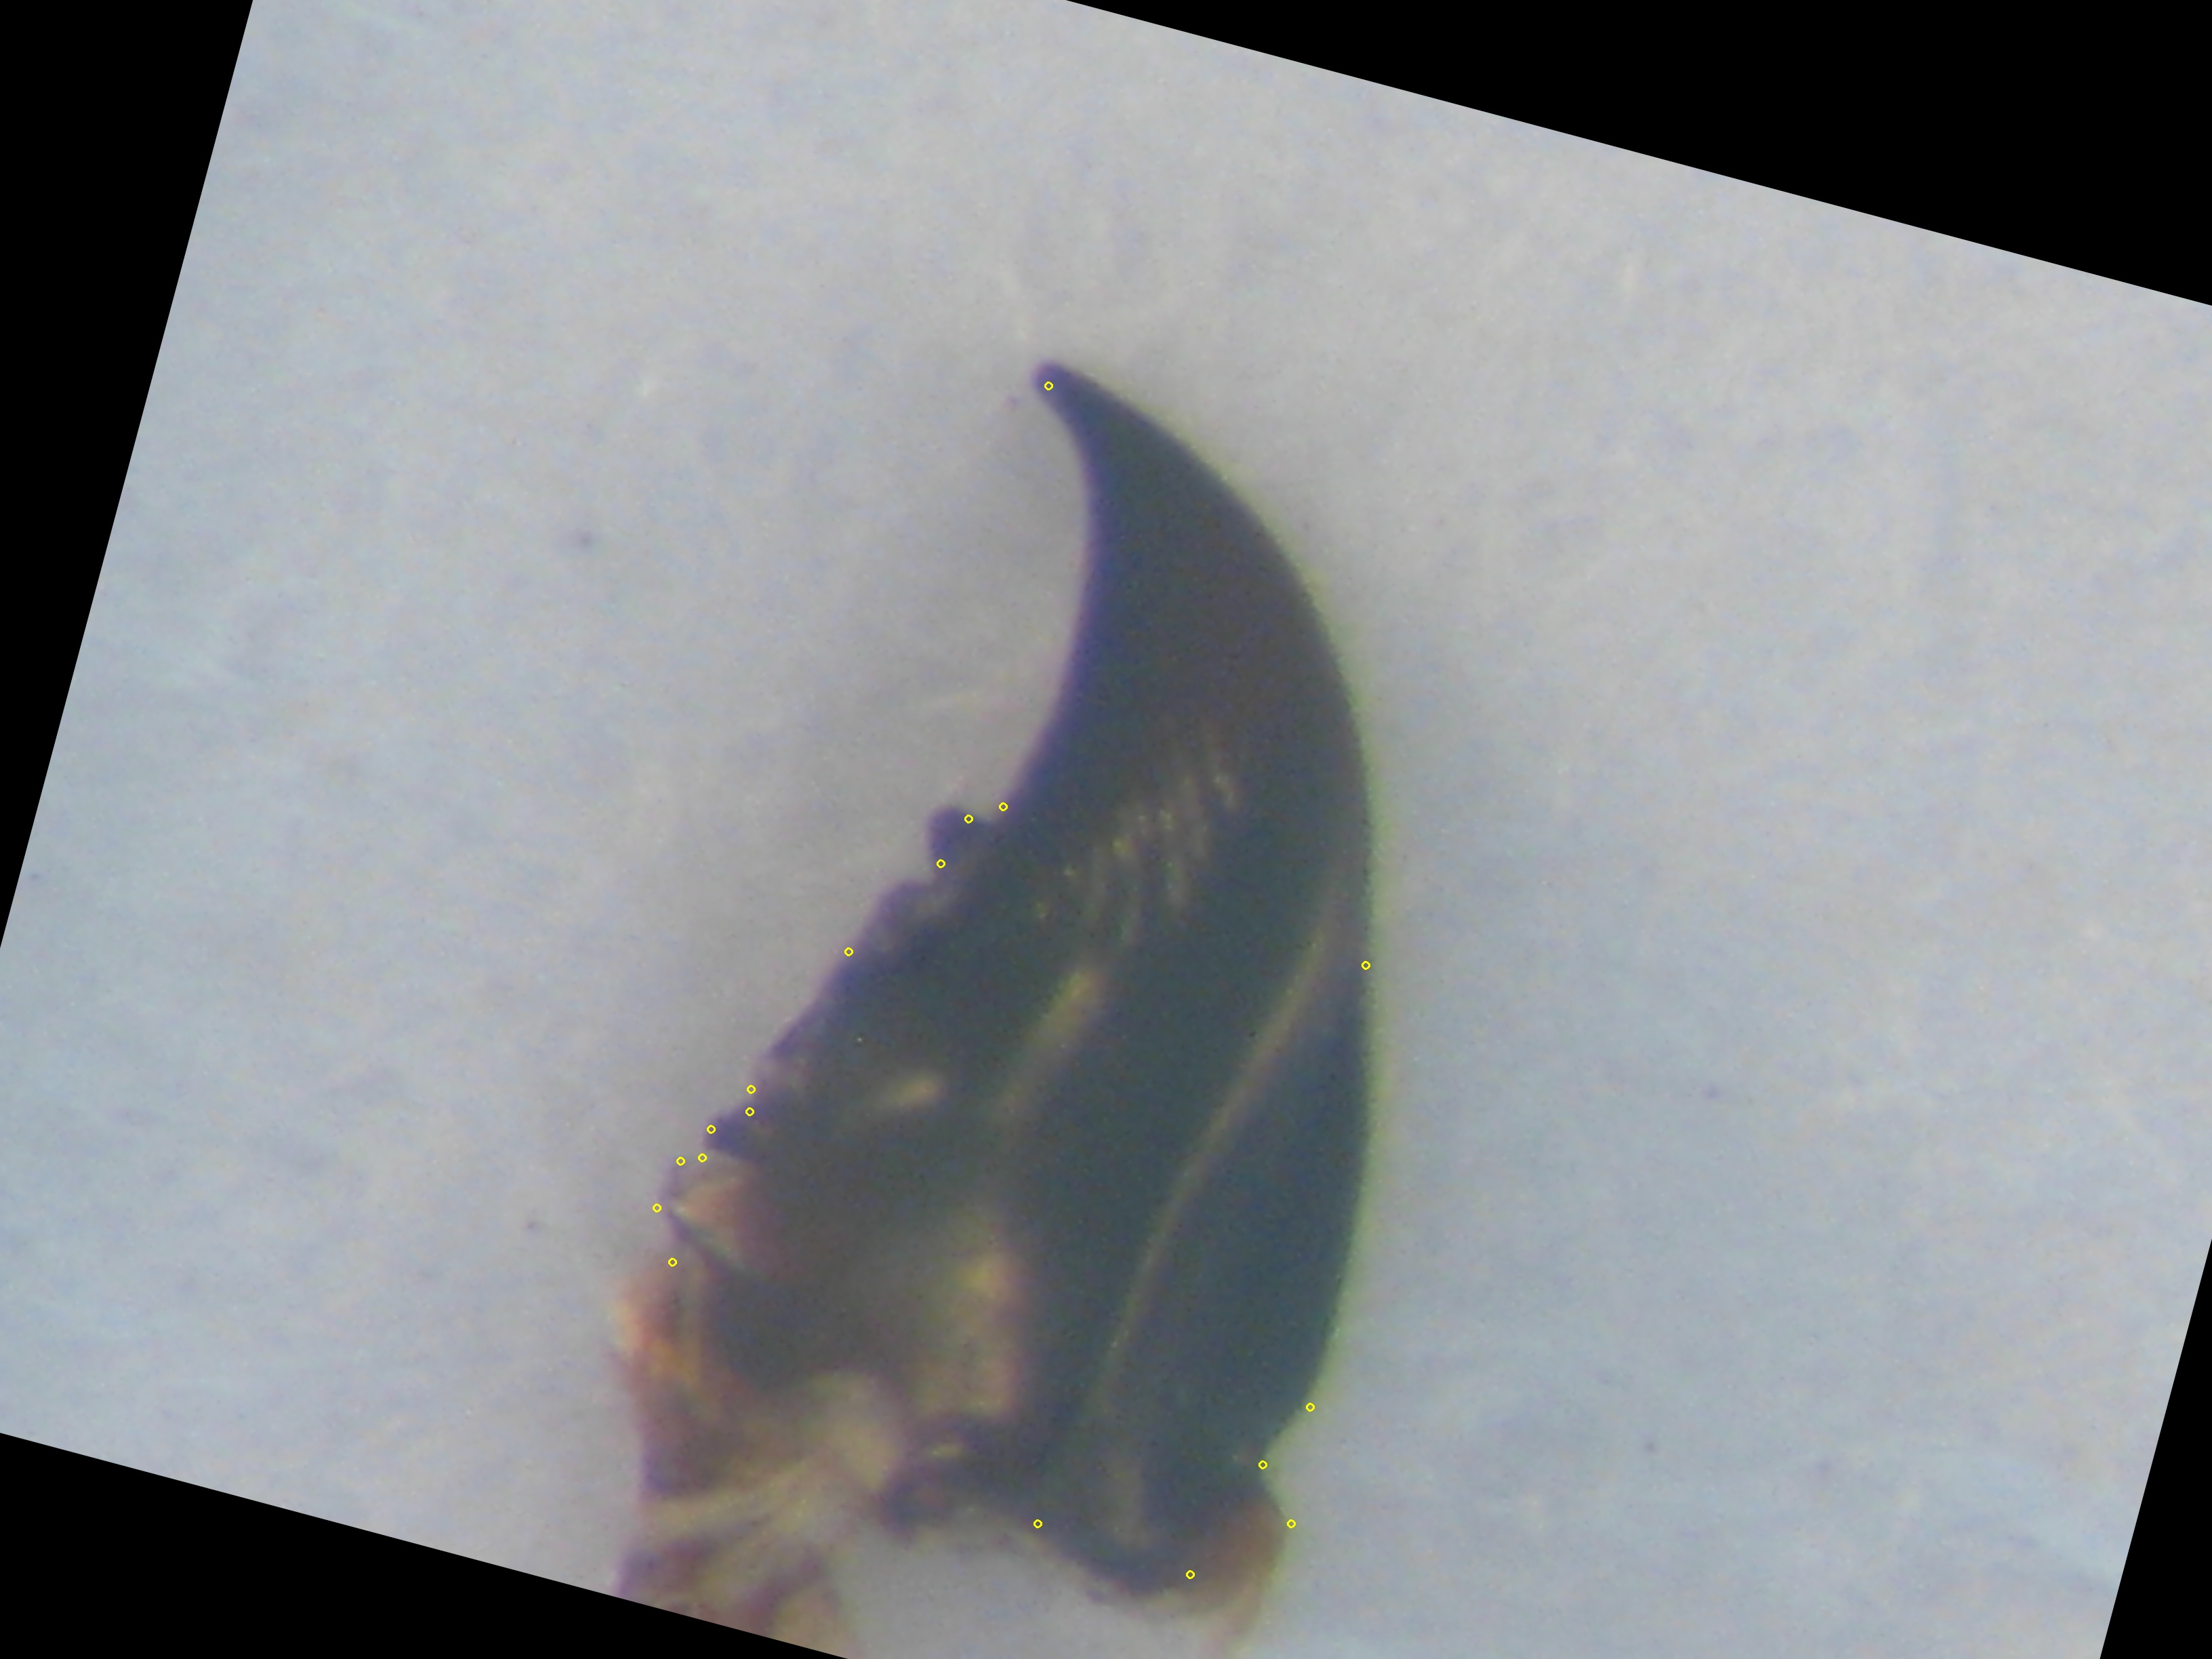
\includegraphics[height=4.5cm]{images/est32.JPG}
	\end{columns}
\end{frame}
\section{Result}
\begin{frame}{Result}
	\begin{itemize}
		\item Dataset: \textit{Mandibule droite} and \textit{mandibule gauche}
		\item Method can be estimated landmarks but the accuracy of the landmarks (compare with original landmarks) is not good.
	\end{itemize}
\end{frame}
\section{References}
\begin{frame}[allowframebreaks]{References}
	\begin{thebibliography}{10}
		\setbeamertemplate{bibliography item}[article]
		\bibitem{palaniswamy}
		Palaniswamy, Sasirekha, Neil A. Thacker, and Christian Peter Klingenberg
		\newblock Automatic identification of landmarks in digital images
		\newblock {\em IET Computer Vision}, 4.4 (2010): 247-260
		
		\setbeamertemplate{bibliography item}[article]		
		\bibitem{pgh}
		Thacker, Neil A., P. A. Riocreux, and R. B. Yates. 
		\newblock "Assessing the completeness properties of pairwise geometric histograms." 
		\newblock{\em Image and Vision Computing}, 13.5 (1995): 423-429.
	\end{thebibliography}
\end{frame}
\begin{frame}[plain]
  \Huge{\centerline{Thank you !}}
\end{frame}
\end{document}